\section{\ourmethod{}}
\subsection{Problem Formulation and Overview}
\noindent
\textbf{Problem formulation.}
In this work, we address \emph{long-horizon robotic imitation learning under partial observability}, where successful task execution requires recalling information no longer present in the current sensory input.
At each time step $t$, the robot receives an observation $o_t$ (e.g., RGB images and proprioception) and executes a low-level action $a_t$.
Let
\[
\tau_t = \{(o_1, a_1), \ldots, (o_{t-1}, a_{t-1}), o_t\}
\]
denote the interaction history up to time $t$.
Additionally, we are given a natural-language task instruction $l$ (e.g., ``put all the bread in the microwave and close the door''), which specifies the high-level goal and is provided to the policy at every time step.
We are given a dataset of expert demonstrations
\[
\mathcal{D} = \{\tau^{(i)}\}_{i=1}^N,
\]
where each trajectory
\[
\tau^{(i)} = \{(o^{(i)}_1, a^{(i)}_1), \ldots, (o^{(i)}_{T_i}, a^{(i)}_{T_i})\}
\]
is collected via teleoperating the robot.
Our aim is to learn a closed-loop visuomotor policy
\[
\pi_\theta(a_t \mid \tau_t, l),
\]
that imitates the expert and performs long-horizon tasks by retrieving and leveraging relevant information from history.

\vspace{0.5em}
\noindent
\textbf{Model architecture overview.}
We parameterize the visuomotor policy $\pi_\theta(a_t \mid \tau_t, l)$ with three main components: 
(i) modality-specific encoders consisting of an observation encoder $g_\theta^{\text{obs}}$ and an action encoder $g_\theta^{\text{act}}$, which map heterogeneous inputs (e.g., RGB images, proprioception, and past actions) into a common latent space,
(ii) a policy backbone $f_\theta$ that performs memory retrieval over the encoded history and processes the information, and
(iii) a task-specific head $h_\theta^{act}$ and $h_\theta^{text}$ that predict low-level control commands and text answers, respectively.

At time step $t$, the current observation is encoded as $x_t = g_\theta^{\text{obs}}(o_t)$ and past actions as $e_i = g_\theta^{\text{act}}(a_i)$ for $i < t$.
The encoded history is
\[
\mathcal{M}_t = \{(x_1, e_1), \ldots, (x_{t-1}, e_{t-1})\}.
\]
Given $\mathcal{M}_t$, the current embedding $x_t$, and the task instruction $l$, the policy backbone $f_\theta$ produces a latent state
\[
z_t = f_\theta(\mathcal{M}_t, x_t, l),
\]
This latent state is passed to two prediction heads: an action head $h_\theta^{\text{act}}(z_t)$ for control and a text prediction head $h_\theta^{\text{text}}(z_t)$ for auxiliary supervision.
% The output of action head provides low-lev
% \[
% \pi_\theta(a_t \mid \tau_t, l) = h_\theta^{\text{act}}(a_t \mid z_t), 
% \quad
% p_\theta(y \mid \tau_t, u) = h_\theta^{\text{text}}(y \mid z_t, u).
% \]

% Using modality-specific encoders allows the policy to process different input modalities while projecting them into a common latent space, enabling the policy backbone to reason jointly over observations, actions, and task instructions. Sharing the weights of the modality-specific encoders and policy backbone enables knowledge sharing across different task objectives.
% The VQA objective and the action prediction objective share the same modality-specific encoders and policy backbone, differing only in their prediction heads.
% This weight sharing encourages the retrieval mechanism to learn representations that are useful both for answering task-relevant questions about the past and for predicting actions.
% As a result, knowledge gained from VQA supervision transfers to action prediction, guiding the policy to retrieve information that is relevant for control.

\vspace{0.5em}
\noindent
\textbf{Method overview.}
A common approach for retrieving information from history is to equip the policy backbone ($f_\theta$) with an \emph{associative memory retrieval mechanism}, typically implemented via learned query--key similarity (\textit{i.e.}, attention)~\cite{vaswani2017attention}.
Such mechanisms provide a general, modality-agnostic way to retrieve information from history, avoiding task-specific designs.

Concretely, the policy backbone $f_\theta$ implements retrieval using a query--key--value formulation.
At each time step $t$, a query vector is computed from the current context,
\[
q_t = f_q(x_t, l),
\]
while each memory element $m_i \in \mathcal{M}_t$ is mapped to a key--value pair,
\[
k_i = f_k(m_i), \qquad v_i = f_v(m_i),
\]
where $f_q$, $f_k$, and $f_v$ are learned functions parameterized by $\theta_q \subset \theta$, $\theta_k \subset \theta$, and $\theta_v \subset \theta$, respectively.
Retrieval is performed by computing similarities between $q_t$ and $\{k_i\}$ and aggregating the corresponding values $\{v_i\}$.
The retrieved features are integrated with the current representation and processed by subsequent model layers.

However, as explained before, directly applying such an attention-based retrieval in long-horizon imitation learning introduces two \emph{key limitations}.
First, because attention aggregates information from all stored history $\mathcal{M}_t$, the policy may attend to task-irrelevant details and incorporate them into decision-making, leading to spurious correlations between past observations and actions.
Second, during closed-loop execution, small prediction errors, compounded by environmental interactions, accumulate over time.
These errors introduce noise into the stored representations, which can degrade latent representation quality, leading to model drift and cascading failures over long horizons.

\ourmethod{} addresses these limitations with two components (Fig.~\ref{fig:method_overview}).
First, we distill task-relevant priors from vision-language models (VLMs) into the policy using automatically generated video question--answer (VQA) supervision.
This supervision encourages the retrieval mechanism to focus on task-relevant information, reducing reliance on irrelevant history (Sec.~\ref{sec:method:vqa-train},~\ref{sec:method:vqa-gen}).
Second, we restrict retrieval to the top-$k$ most relevant memory entries at each time step.
This sparsification limits the influence of accumulated error during closed-loop execution, leading to robust long-horizon control (Sec .~\ref{sec:method:topk}).

% We implement these ideas by training a single visuomotor policy with a shared backbone that jointly (i) imitates expert actions and (ii) answers VQA queries about the trajectory history.
% The backbone $f_\theta$ contains the memory retrieval mechanism and is shared across outputs.
% Both objectives use the same top-$k$ sparsified retrieval, encouraging the policy to retrieve and condition only on a subset of useful information.
% 
% \ourmethod{} addresses both limitations with two components (Fig.~\ref{fig:method_overview}).
% First, we distill task-relevant priors from vision-language models (VLMs) into the policy using automatically generated video question--answer (VQA) supervision, which explicitly guides the memory retrieval mechanism toward information relevant to the task and reduces spurious correlations.
% Second, to improve performance in closed-loop execution, we restrict the policy to conditioning only on the top-$k$ most relevant information from the history at each time step.
% This explicit sparsification prevents the policy from repeatedly conditioning on large amounts of noisy information, mitigating long-horizon drift.

Concretely, \ourmethod{} trains a single visuomotor policy that jointly (i) imitates expert actions and (ii) answers VQA queries about the trajectory history.
Both objectives share the same modality-specific encoders $g_\theta$ and a common backbone $f_\theta$ that contains the memory retrieval mechanism, differing only in their prediction heads.
Top-$k$ sparsification is applied to retrieval for both objectives, encouraging the policy to condition only on a subset of relevant memory entries.
This shared training and policy weights encourages the retrieval mechanism to learn representations that are useful for both answering questions about the past and predicting actions.
As a result, supervision from VQA transfers to action prediction, guiding the policy to retrieve information relevant for control.

\subsection{Distilling Vision-Language Model Priors via Video Question--Answering}\label{sec:method:vqa-train}

Vision-language models encode rich priors about scenes, objects, activities, and semantics to understand task instructions, making them a useful source of guidance for identifying task-relevant information in trajectories.
However, because VLMs are not grounded in action prediction, these priors alone do not capture all the information required for effective low-level control.
\ourmethod{} therefore distills priors from VLMs into the policy while grounding them through imitation learning.

\vspace{0.5em}
\noindent
\textbf{Video question--answering as retrieval supervision.}
% Let $\mathcal{M}_t$ denote the encoded interaction history defined earlier, consisting of representations derived from past observations and actions.
% At time $t$, the observation encoder produces the current embedding $x_t = g_\theta^{\text{obs}}(o_t)$.
% Conditioned on the encoded history $\mathcal{M}_t$, the current observation embedding $x_t$, and the task instruction $l$, the policy backbone $f_\theta$ produces a latent query vector
% \[
% q_t = f_q(\mathcal{M}_t, x_t, l),
% \]
% and retrieves a context vector $c_t$ from $\mathcal{M}_t$ using a learned query--key mechanism (described in Section~\ref{sec:topk}).
In standard end-to-end imitation learning, the retrieval mechanism is trained solely through the action prediction objective.
\ourmethod{} additionally supervises the retrieval process using the video question--answering objective.
Specifically, we generate VQA pairs $(u, v)$, where $u$ is a text-based question probing task-relevant information from the trajectory history (e.g., object locations, object relations, event ordering, or subgoal progress), and $v$ is the corresponding answer.
For VQA supervision, the policy backbone is conditioned on the encoded history $\mathcal{M}_t$, the current observation embedding $x_t$, and the question $u$, and the answer is predicted via a VQA head:
\begin{equation}
    \hat{v} \sim \pi_\theta^{\text{vqa}}(v \mid \mathcal{M}_t, x_t, u),
\end{equation}
where $\pi_\theta^{\text{vqa}}$ consists of the shared observation $g_\theta^{\text{obs}}$, action encoder $g_\theta^{\text{act}}$, policy backbone $f_\theta$ (including the retrieval mechanism) with the action prediction objective, and a text prediction head $h_\theta^{text}$.

To answer $u$, the policy must retrieve the specific information from the history that supports the answer.
Since the questions are generated using vision-language models and tailored to the task, this objective injects task-relevant priors into the retrieval mechanism, providing direct supervision on what information should be retrieved.

\vspace{0.5em}
\noindent
\textbf{Joint grounding through imitation learning.}
While VQA supervision guides retrieval toward task-relevant information, it does not by itself ensure that the retrieved information is sufficient for low-level control.
We therefore jointly train the policy using an imitation learning objective:
\begin{equation}
    \mathcal{L}_{\text{IL}}(\theta)
    = \mathbb{E}_{(\tau_t, s, a_t^*) \sim \mathcal{D}}
    \left[-\log \pi_\theta^{\text{act}}(a_t^* \mid \tau_t, l)\right],
\end{equation}
where $a_t^*$ denotes the expert action.
We also define a VQA loss over the generated dataset $\widetilde{\mathcal{D}}$:
\begin{equation}
    \mathcal{L}_{\text{VQA}}(\theta)
    = \mathbb{E}_{(\tau_t, s, u, v) \sim \widetilde{\mathcal{D}}}
    \left[-\log \pi_\theta^{\text{vqa}}(v \mid \tau_t, u)\right].
\end{equation}
The final training objective is
\begin{equation}
    \mathcal{L}(\theta)
    = \mathcal{L}_{\text{IL}}(\theta)
    + \lambda \mathcal{L}_{\text{VQA}}(\theta),
\end{equation}
where $\lambda$ balances imitation and VQA supervision.
This joint training ensures that VQA provides informative priors about what information from the history should be retrieved, while imitation learning grounds retrieval in expert action prediction.

\subsection{Generating VQA Data from Long-Horizon Trajectories}\label{sec:method:vqa-gen}
\begin{figure}[htbp]
    \centering
    \vspace{-10pt}
    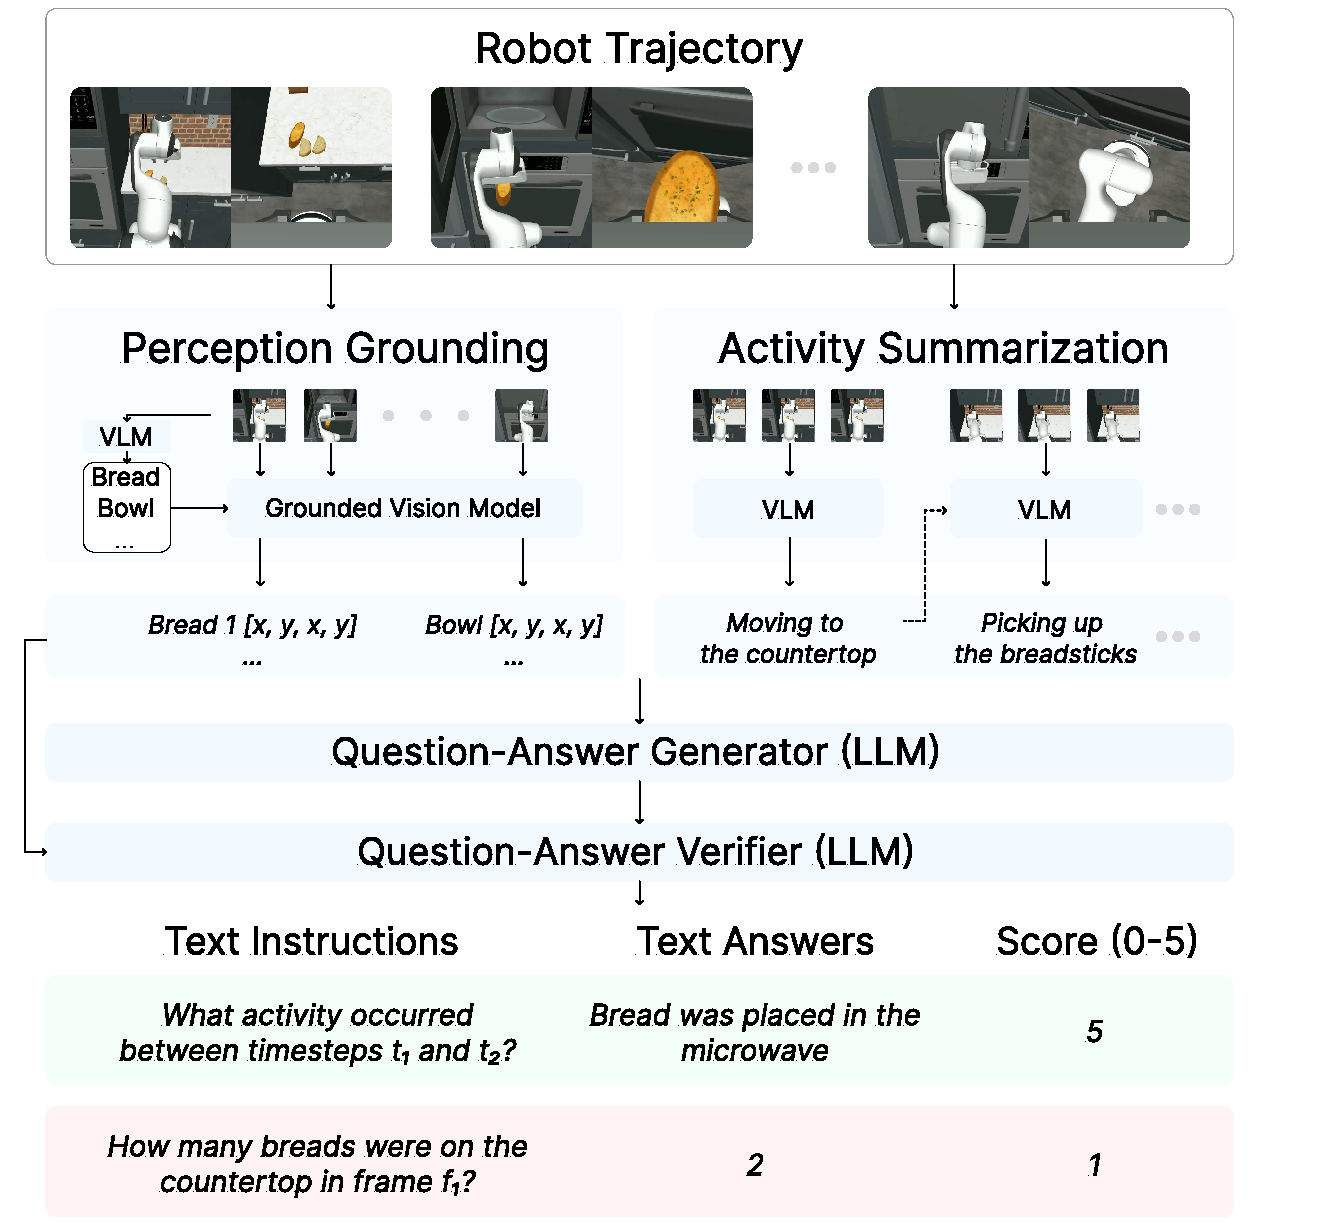
\includegraphics[width=0.5\textwidth]{figures/vqa-generation.pdf}
    \vspace{-15pt}
    \caption{\textbf{Overview of video question-answer generation for knowledge distillation.} Images are first converted to text using a grounded vision model, and trajectories are summarized with each subtask and corresponding frame numbers. An LLM generates task-relevant question-answer pairs from these summaries and the task description, which are then verified for correctness and relevance, filtering out about $20\%$ of the data.}
    \label{fig:vqa_generation}
    \vspace{-15pt}
\end{figure}

Generating accurate VQA supervision for long-horizon robot trajectories is challenging. Single VLM calls over high-dimensional visual information often produce incorrect or hallucinated question-answer pairs, likely because state-of-the-art VLMs struggle to process long-context visual information coherently. To address this, we employ a multi-stage generation pipeline that produces high-quality supervision (Fig.~\ref{fig:vqa_generation}).

\textit{(i) Trajectory-to-text summarization.}
Given a trajectory segment, we construct a textual description that captures scene elements (e.g., object identities and locations) and activity descriptions (e.g., ``the robot opened the drawer and placed the mug inside'').
To do so, we combine information from different specialized vision models, such as object detectors for spatial cues and VLMs for higher-level activity descriptions, and consolidate them into a single text representation of the trajectory.
This consolidation is performed only to generate questions and answers that provide retrieval priors; the information itself may not be sufficient to capture all the information required by the policy to predict low-level actions.

\textit{(ii) Question and answer synthesis.}
From the consolidated text, we synthesize questions that probe memory requirements relevant to the task.
We observe that language models tend to bias questions toward task-relevant information present in the initial portion of a trajectory.
To mitigate this bias, we explicitly prompt the language model to generate a question corresponding to a specific frame index, randomly sampled from the trajectory.
The model is also allowed to return ``N/A'' if no task-relevant information is present at the specified frame. We ask the language model to also generate the answer corresponding to the question.

\textit{(iii) Automatic filtering for correctness and relevance.}
Generated VQA pairs may contain incorrect or be weakly task-relevant or labeled as ``N/A''.
To improve data quality, we use an additional language model to rate each pair on correctness with respect to the trajectory description and relevance to the task.
Pairs with low scores are filtered out.
The remaining set forms $\widetilde{\mathcal{D}}$, which is used for training.

% \begin{figure}[htbp]
%     \centering
%     \includegraphics[width=0.48\textwidth]{figures/rw_task_figure.pdf}
%     \caption{Visualization of real-world tasks.}
%     \label{fig:pull_figure}
% \end{figure}

\begin{figure*}[t]
    % \vspace{0.5cm}
    \centering
    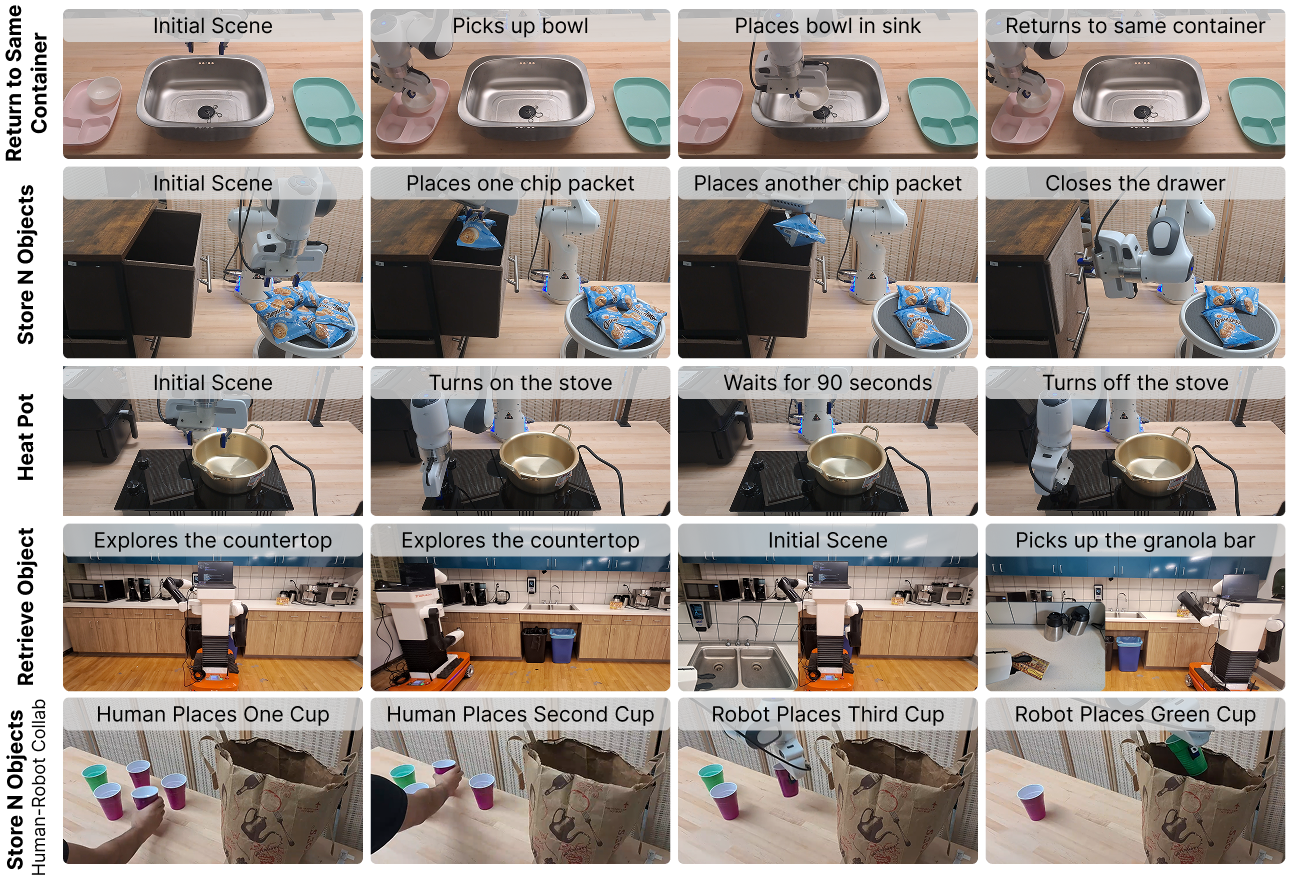
\includegraphics[width=0.98\textwidth]{figures/rw_task_figure_5.png}
    \vspace{-10pt}
    \caption{\textbf{Visualization of real-world tasks.} We evaluate \ourmethod{} in four stationary and mobile manipulation tasks, including a human-robot collaborative task (\textit{rows}) with strong partial observability, where the agent needs to retrieve different types of information from memory. The pictures in each column depict a different phase of the task.}
    \label{fig:rw_task_viz}
    \vspace{-10pt}
\end{figure*}

\subsection{Reducing Model Drift with Top-$K$ Attention Sparsification}
\label{sec:method:topk}
Even with improved retrieval supervision, long-horizon closed-loop execution remains susceptible to error accumulation.
In offline imitation learning, policies are trained on expert trajectories but must execute actions based on their own predictions at test time.
Small prediction errors can lead to future observations that deviate from the expected observations, leading to compounding errors over time.
Conditioning on large amounts of information from memory can further exacerbate this effect by repeatedly incorporating noisy information, resulting in cascading failures over long horizons.

To mitigate this issue, \ourmethod{} explicitly limits how much information from the history the policy can condition on at each time step.
Rather than attending to all available information, we first identify the information most relevant to the current decision and restrict retrieval to only these elements.
This allows the policy to focus on important information while reducing the effect of accumulated error in memory.

Concretely, let $\{m_i\}_{i=1}^{|\mathcal{M}_t|}$ denote candidate information extracted from the history, with keys $k_i = f_k(m_i)$ and values $v_i = f_v(m_i)$.
Given a query $q_t$, standard attention computes scores $s_i = \langle q_t, k_i \rangle$ and forms a weighted sum over all values.
In top-$k$ sparsification, we instead select
\begin{equation}
    \mathcal{I}_k = \mathrm{TopK}(\{s_i\}_{i=1}^{|\mathcal{M}_t|}, k),
\end{equation}
corresponding to the $k$ most relevant elements, and compute attention only over this subset with all elements outside $\mathcal{I}_k$ receive zero weight:
\begin{equation}
    c_t = \sum_{i \in \mathcal{I}_k}
    \frac{\exp(s_i)}{\sum_{j \in \mathcal{I}_k} \exp(s_j)} v_i.
\end{equation}

Since the top-$k$ operation is non-differentiable, we employ a straight-through estimator during training.
Intuitively, at each training step, the policy retrieves the top-$k$ elements based on the query--key similarity using the current model weights.
If the retrieved information improves action prediction or VQA accuracy, gradients flowing through the attention output increase the corresponding query--key similarities, reinforcing the selection of useful information.
Conversely, elements that do not contribute meaningfully receive weaker updates and are less likely to be selected in future steps.

To summarize, \ourmethod{} combines VQA-based distillation of informative VLM priors, which encourages task-relevant retrieval and reduces spurious correlations, with top-$k$ sparse attention, which limits error accumulation and mitigates model drift, yielding a policy that is effective for long-horizon, partially observable tasks.
